\section{Nhận diện Tư thế Người và Phát hiện Té ngã}
\label{sec:pose_fall_system}

Mục này trình bày tổng quan về nhận diện tư thế người, giải pháp thời gian thực MediaPipe Pose, xây dựng thuật toán phát hiện té ngã dựa trên đặc trưng động học và tư thế, cùng mô tả chi tiết hệ thống tích hợp.

\subsection{Nhận diện Tư thế Người}

Nhận diện tư thế người là một lĩnh vực then chốt trong thị giác máy tính, nhằm xác định vị trí và hướng các khớp và bộ phận cơ thể từ hình ảnh hoặc chuỗi video. Khả năng này là nền tảng cho các ứng dụng giám sát an toàn, phân tích chuyển động, và nhận diện hành vi bất thường (như té ngã).


\begin{figure}[H]
    \centering
    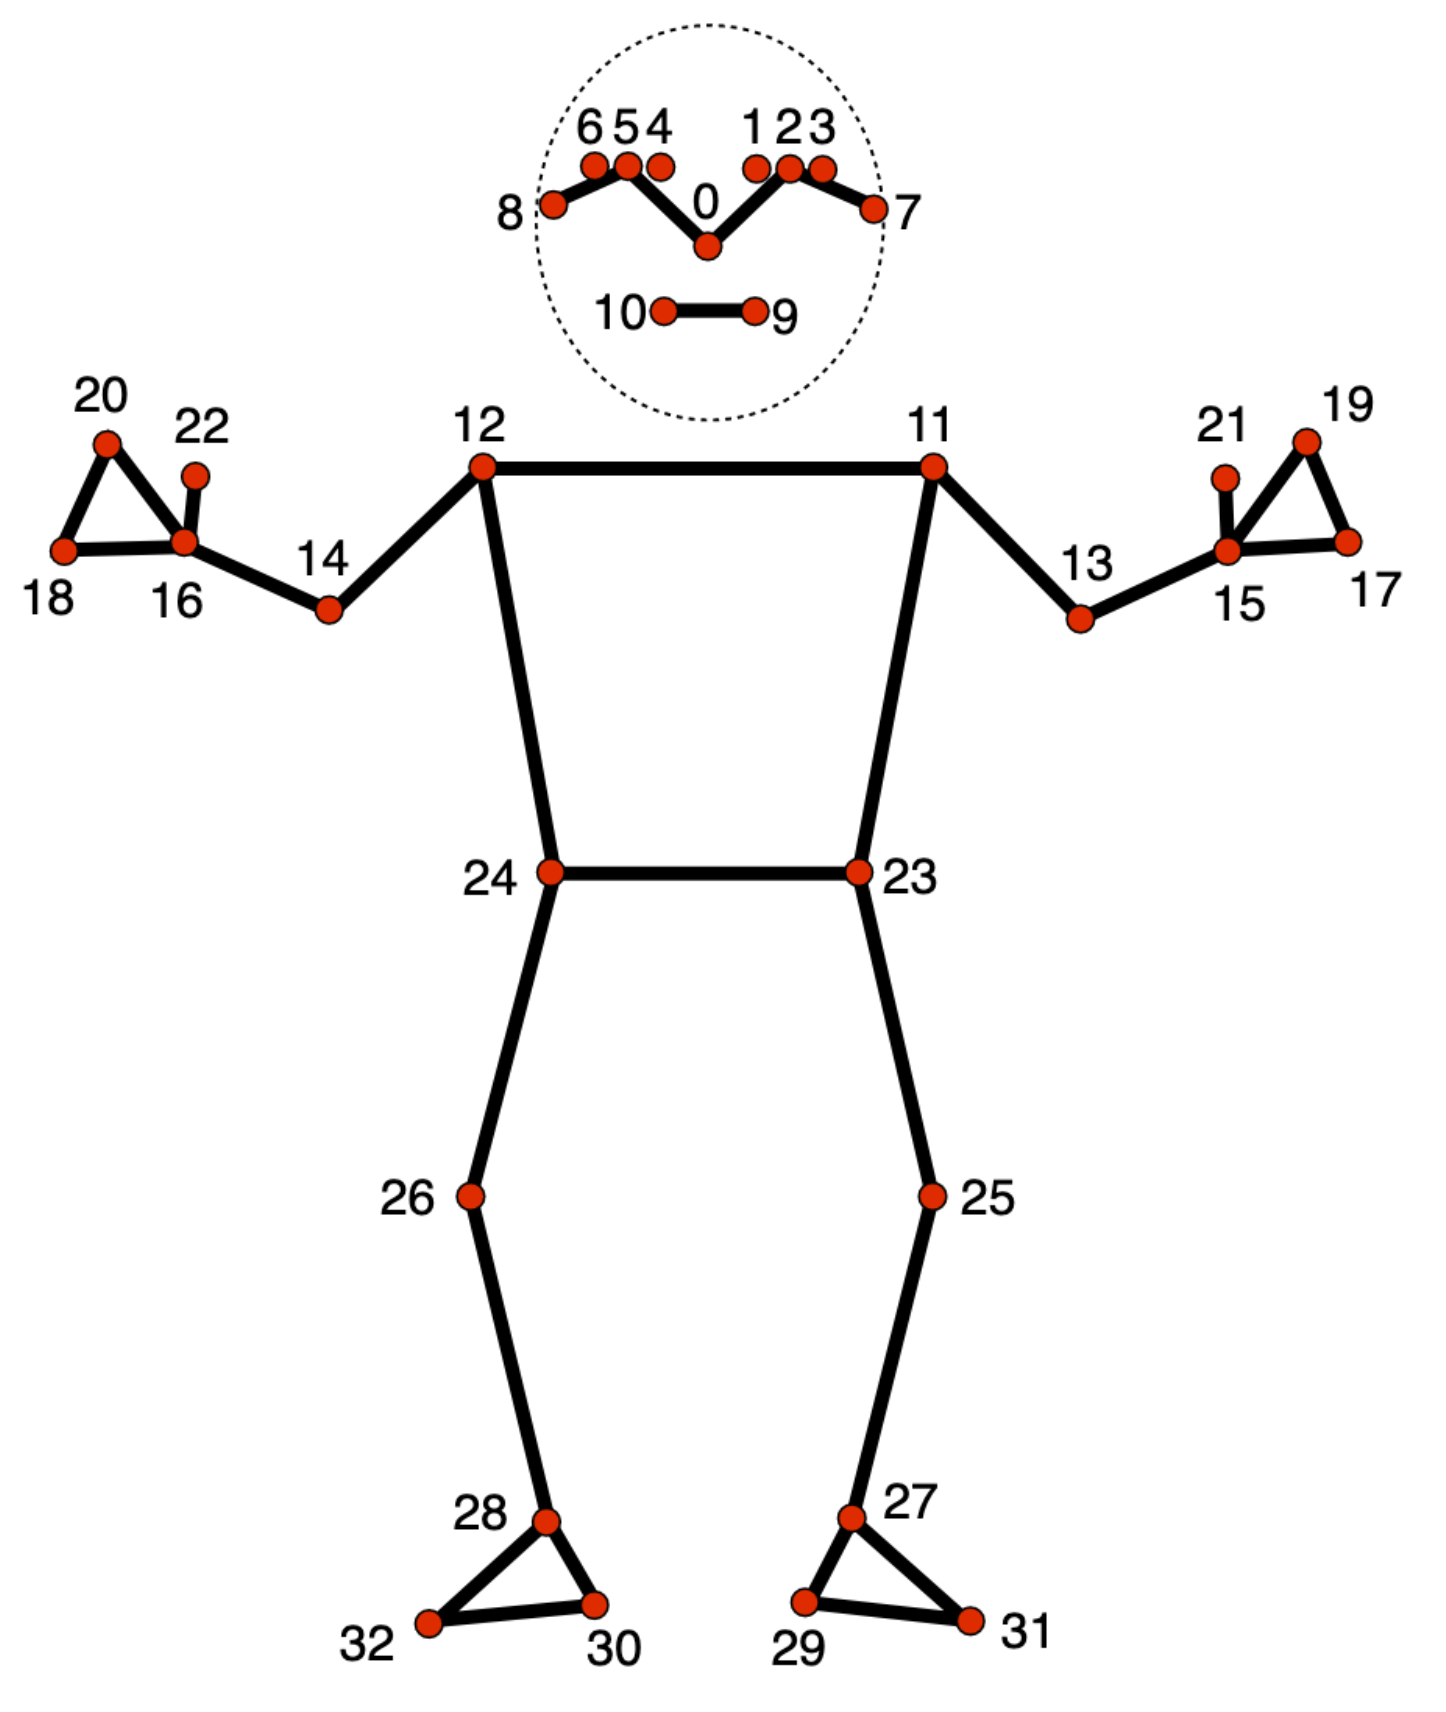
\includegraphics[width=0.5\textwidth]{pose_landmarks_index.png}
    \caption{Minh họa 33 điểm mốc (keypoints) tiêu chuẩn trong nhận diện tư thế người.}
\end{figure}

\subsubsection{Khái niệm và Định nghĩa}

Pose Estimation ước lượng vị trí của các bộ phận cơ thể trong không gian 2D hoặc 3D, được biểu diễn qua tập hợp các \textbf{keypoints}:
\begin{equation}
\mathcal{K} = \{k_1, k_2, ..., k_n\}, \quad k_i = (x_i, y_i, z_i, c_i)
\end{equation}
trong đó $(x_i, y_i, z_i)$ là tọa độ không gian (với $z_i$ là tọa độ chiều sâu tương đối) và $c_i$ là độ tin cậy (\textbf{confidence score}) của keypoint thứ $i$.

\paragraph{Phân loại Phương pháp HPE:}
\begin{itemize}
    \item \textbf{Top-down Approach:} Đầu tiên phát hiện đối tượng người, sau đó ước lượng keypoints cho từng hộp giới hạn (bounding box) của người. (VD: Mask R-CNN, MediaPipe).
    \item \textbf{Bottom-up Approach:} Đầu tiên phát hiện tất cả các keypoints, sau đó nhóm chúng lại để tạo thành tư thế của từng người. (VD: OpenPose).
\end{itemize}

\subsection{MediaPipe Pose Estimation cho Ứng dụng Thời gian thực}

MediaPipe Pose, dựa trên mô hình BlazePose của Google, được tối ưu hóa để cung cấp giải pháp HPE 3D nhanh và chính xác trong môi trường thời gian thực trên nhiều nền tảng (Mobile, Web, Desktop).

\subsubsection{Kiến trúc xử lý Graph-based}

MediaPipe sử dụng kiến trúc xử lý dữ liệu dựa trên đồ thị, nơi các nhiệm vụ được tổ chức thành một chuỗi các module:
\begin{itemize}
    \item \textbf{Nodes:} Các module xử lý độc lập thực hiện các nhiệm vụ cụ thể (VD: Phát hiện đối tượng, Ước lượng điểm mốc).
    \item \textbf{Edges (Packet Stream):} Các luồng dữ liệu được truyền tải giữa các Nodes, đảm bảo đồng bộ hóa và nhất quán dữ liệu giữa các bước.
\end{itemize}

\subsubsection{Các thành phần Mô hình Chính}

\paragraph{Pose Detection Model:} Nhiệm vụ là phát hiện sự hiện diện và xác định \textbf{Vùng quan tâm (ROI)} chứa người trong khung hình.
\begin{itemize}
    \item Input: Khung hình RGB.
    \item Output: Bounding box và xác suất hiện diện của người.
\end{itemize}

\paragraph{Pose Landmark Model:} Mô hình ước lượng các điểm mốc chính xác trên ROI đã xác định.
\begin{itemize}
    \item Output: 33 keypoints 3D $(x, y, z, visibility)$.
    \item Hàm mất mát tổng hợp:
    \begin{equation}
    \mathcal{L}_{\text{total}} = \lambda_1 \mathcal{L}_{\text{coord}} + \lambda_2 \mathcal{L}_{\text{confidence}} + \lambda_3 \mathcal{L}_{\text{depth}}
    \end{equation}
\end{itemize}

\paragraph{Pose Tracking Model:} Dự đoán ROI cho khung hình tiếp theo dựa trên pose hiện tại. Việc này giúp giảm đáng kể chi phí tính toán bằng cách tránh chạy mô hình phát hiện đầy đủ ở mỗi khung hình.

\subsubsection{Thuật toán Hậu xử lý (Post-processing)}

\paragraph{Temporal Smoothing (One Euro Filter):} Áp dụng bộ lọc thời gian để làm mịn tín hiệu tọa độ keypoint qua các khung hình, loại bỏ nhiễu và tăng độ ổn định của chuyển động ước tính.

\paragraph{3D Coordinate Estimation:} Chiều sâu tương đối $z$ được chuẩn hóa dựa trên kích thước cơ thể (thường là khoảng cách giữa hông).

\subsection{Thuật toán Phát hiện Té ngã Multi-stage}

Hệ thống phát hiện té ngã sử dụng các đặc trưng động học và tư thế được trích xuất từ dữ liệu keypoints 3D (từ MediaPipe) để đưa ra quyết định qua nhiều giai đoạn. $\Delta t$ được định nghĩa là thời gian trôi qua giữa hai khung hình liên tiếp ($1/FPS$).

\subsubsection{Trích xuất Đặc trưng Sinh học}

\paragraph{Đặc trưng Động học:} Phản ánh tốc độ và gia tốc trong quá trình té ngã.
\begin{itemize}
    \item \textbf{Vận tốc COM ($\vec{v}_{\text{COM}}$) và Gia tốc COM ($a_{\text{total}}$):}
    \begin{align}
    \vec{v}_{\text{COM}}(t) &= \frac{\vec{p}_{\text{COM}}(t) - \vec{p}_{\text{COM}}(t-\Delta t)}{\Delta t} \\
    \vec{p}_{\text{COM}} &= \frac{\sum_i w_i \vec{p}_i c_i}{\sum_i w_i c_i} \quad (\text{Với } w_i \text{ là trọng số khối lượng sinh học}) \\
    a_{\text{total}}(t) &= \frac{\|\vec{v}_{\text{COM}}(t) - \vec{v}_{\text{COM}}(t-\Delta t)\|}{\Delta t}
    \end{align}
\end{itemize}

\paragraph{Đặc trưng Tư thế:} Phản ánh hình dạng cơ thể và độ cao sau khi té ngã.
\begin{itemize}
    \item \textbf{Tỷ lệ cạnh (Aspect Ratio - AR):} Tỷ lệ giữa chiều rộng và chiều cao của hộp giới hạn người, tăng vọt khi người nằm ngang.
    \item \textbf{Góc Nghiêng Cơ thể ($\theta_{\text{body}}$):} Góc tạo bởi trục cơ thể (vai-hông) so với phương thẳng đứng.
    \item \textbf{Độ giảm chiều cao ($\Delta h_{\text{head}}$):} Sự thay đổi vị trí của đầu so với trạng thái ban đầu.
\end{itemize}

\subsubsection{Thuật toán Phát hiện Té ngã Ba Giai đoạn}

\paragraph{Stage 1: Phát hiện Sớm}
Kiểm tra các dấu hiệu ban đầu của sự mất kiểm soát, chủ yếu dựa vào tốc độ và gia tốc của Trung tâm Khối lượng (COM).

\paragraph{Stage 2: Xác nhận Sự kiện Té ngã}
Nếu Stage 1 là True, kiểm tra các đặc trưng tư thế (AR, $\theta_{\text{body}}$) để xác nhận trạng thái cơ thể chuyển từ đứng/đi sang nằm ngang.

\paragraph{Stage 3: Kiểm tra Bất động sau té ngã}
Sau khi té ngã được xác nhận (Stage 2 là True), hệ thống theo dõi mức độ chuyển động trong một khoảng thời gian ($T_{\text{window}}$). Nếu sự chuyển động thấp hơn ngưỡng $M_{th}$ trong thời gian dài, cảnh báo được kích hoạt, loại trừ các trường hợp ngồi hoặc nằm chủ động.
